\documentclass[a4paper,12pt]{article}
\usepackage[utf8]{inputenc}
\usepackage[ngerman]{babel}
\usepackage[top=1in, bottom=1.25in, left=1.25in, right=1.25in]{geometry}
\usepackage{minted}
\usepackage{blindtext}
\usepackage{fancyhdr}
\usepackage{titling}
\usepackage{amssymb}
\usepackage{mathtools}
\usepackage{systeme}
\usepackage{tikz}

\usepackage{graphicx}
\graphicspath{ {./} }
\usetikzlibrary{calc,tikzmark}


\renewcommand{\footrulewidth}{0.4pt}

\setlength\headheight{15pt}
\setlength{\parskip}{1em}

\title{Lineare Algebra 1, Blatt 3}
\author{
    Ben Krogmann
    \and
    Eli Kogan-Wang
}
\date{\today}

\pagestyle{fancy}
\fancyhf{}
\lhead{\thetitle}
\rhead{\thedate}
\lfoot{\theauthor}
\rfoot{Seite \thepage}


\begin{document}
\maketitle
\thispagestyle{fancy}

\paragraph{Aufgabe 12}
% ./Lina1Blatt3Aufgabe12.jpg
% ./Lina1Blatt3Aufgabe12b.jpg
%itemized list
\begin{itemize}
    \item % image
          1. 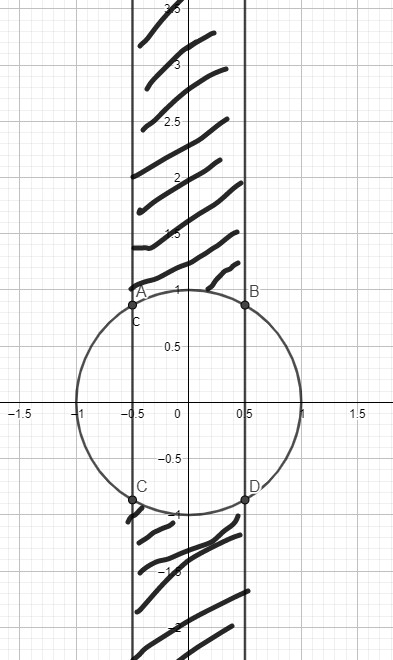
\includegraphics{Lina1Blatt3Aufgabe12}
    \item % image
          2. 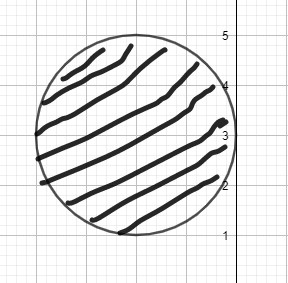
\includegraphics{Lina1Blatt3Aufgabe12b}
\end{itemize}



\paragraph{Aufgabe 13}
\begin{itemize}
    \item $(1+i)^{10}=((1+i)^2)^5=(1+2i-1)^5=2^5i^5=2^5i$
    \item $(1-\sqrt3i)^6=(2(\frac12-\frac{\sqrt{3}}2i))^6=2^6(\cos(\frac{5\pi}3)+i\sin(\frac{5\pi}3))^6=2^6(\cos(10\pi)+i\sin(10\pi))=2^6(\cos(0)+i\sin(0))=2^6(1)=2^6$
    \item $(\frac{\sqrt3+i}{1-i})^{12}=(\frac{(\sqrt3+i)(1+i)}{(1-i)(1+i)})^{12}=(\frac{\sqrt3+i+\sqrt3i+i^2}{2})^{12}=(\frac{(\sqrt3-1)+i(1+\sqrt3)}{2})^{12}\\=\frac1{2^{12}}((\sqrt3-1)+i(\sqrt3+1))^{12}\overset*=\frac{\sqrt8^{12}}{2^{12}}(\frac{\sqrt3+1}{\sqrt8}+\frac{\sqrt3-1}{\sqrt8}i)^{12}\\=\frac{8^6}{2^{12}}(\cos(\frac\pi{12})+i\sin(\frac\pi{12}))^{12}=\frac{(2^{3})^6)}{2^{12}}(\cos(\pi)+i\sin(\pi))=\frac{2^{18}}{2^{12}}(i)=2^6i$
    \item $\sqrt{(\sqrt3+1)^2+(\sqrt3-1)^2}=\sqrt{3+2\sqrt3+1+3-2\sqrt3+1}=\sqrt8$
    \item $(\frac{\sqrt3-i}{\sqrt3+i})^{2021}=(\frac{(\sqrt3-i)(\sqrt3-i)}{(\sqrt3+i)(\sqrt3-i)})^{2021}=(\frac{3-2\sqrt3i-1}{4})^{2021}=(\frac{1-\sqrt3i}{2})^{2021}=(\cos(\frac{5\pi}3)+i\sin(\frac{5\pi}3))^{2021}=\cos(\frac{10105\pi}{3})+i\sin(\frac{10105\pi}{3})=\cos(3368\pi+\frac\pi3)+i\sin(3368\pi+\frac\pi3)=\cos(\frac\pi3)+i\sin(\frac\pi3)=\frac12+\frac{\sqrt{3}}2i$
\end{itemize}


\paragraph{Aufgabe 14}
$z\in\mathbb C:z^2=\overline z$

$\{z\in\mathbb C:|z|=1\}$

\paragraph{Aufgabe 15}
$K:=\{a+\sqrt3ib|a,b\in\mathbb Q\}\subseteq\mathbb C$

\paragraph{Aufgabe 16}
$\forall \theta\in\mathbb R,z\in\mathbb C\backslash\{0\},n\in\mathbb N:z+\frac1z=2\cos(\theta)$

z.z.
$z^n+z^{-n}=2\cos(n\theta)$


\paragraph{Aufgabe 17}
\subparagraph{(1)}
$\begin{aligned}
                                                                      & \begin{pmatrix}3-i&4+2i&|&2+6i\\4+2i&-2-3i&|&5+4i\end{pmatrix}                                              \\
        \overset{I\cdot(3+i),II\cdot(4-2i)}\rightsquigarrow           & \begin{pmatrix}(3-i)(3+i)&(4+2i)(3+i)&|&(2+6i)(3+i)\\(4+2i)(4-2i)&(-2-3i)(4-2i)&|&(5+4i)(4-2i)\end{pmatrix} \\
        \overset{}\rightsquigarrow                                    & \begin{pmatrix}10&12+6i+4i-2&|&6+18i+2i-6\\20&-8-12i+4i-6&|&20+16i-10i+8\end{pmatrix}                       \\
        \overset{I\cdot(\frac1{10}),II\cdot(\frac12)}\rightsquigarrow & \begin{pmatrix}1&1+i&|&2i\\10&-7-4i&|&14+3i\end{pmatrix}                                                    \\
        \overset{II-10I}\rightsquigarrow                              & \begin{pmatrix}1&1+i&|&2i\\0&-17-14i&|&14-17i\end{pmatrix}                                                  \\
        \overset{II\cdot(-17+14i)}\rightsquigarrow                    & \begin{pmatrix}1&1+i&|&2i\\0&(-17-14i)(-17+14i)&|&(14-17i)(-17+14i)\end{pmatrix}                            \\
        \overset{II-2I}\rightsquigarrow                               & \begin{pmatrix}1&1+i&|&2i\\0&485&|&485i\end{pmatrix}                                                        \\
        \overset{II-2I}\rightsquigarrow                               & \begin{pmatrix}1&1+i&|&2i\\0&1&|&i\end{pmatrix}                                                             \\
        \overset{I-(1+i)II}\rightsquigarrow                           & \begin{pmatrix}1&0&|&1+i\\0&1&|&i\end{pmatrix}                                                              \\
    \end{aligned}$

$\begin{pmatrix}x\\y\end{pmatrix}=\begin{pmatrix}1+i\\i\end{pmatrix}$

\subparagraph{(2)}
$\begin{aligned}
                                                       & \begin{pmatrix}1&i&-2&|&10\\1&-1&2i&|&20\\i&3i&-1-i&|&30\end{pmatrix}           \\
        \overset{II-I,III-i\cdot I}\rightsquigarrow    & \begin{pmatrix}1&i&-2&|&10\\0&-1-i&2i+2&|&10\\0&3i+1&-1+i&|&30-10i\end{pmatrix} \\
        \overset{II\cdot(-1+i)}\rightsquigarrow        & \begin{pmatrix}1&i&-2&|&10\\0&2&-4&|&-10+10i\\0&3i+1&-1+i&|&30-10i\end{pmatrix} \\
        \overset{II\cdot\frac12}\rightsquigarrow       & \begin{pmatrix}1&i&-2&|&10\\0&1&-2&|&-5+5i\\0&3i+1&-1+i&|&30-10i\end{pmatrix}   \\
        \overset{III-(3i+1)II}\rightsquigarrow         & \begin{pmatrix}1&i&-2&|&10\\0&1&-2&|&-5+5i\\0&0&7i+1&|&50\end{pmatrix}          \\
        \overset{III\cdot(1-7i)}\rightsquigarrow       & \begin{pmatrix}1&i&-2&|&10\\0&1&-2&|&-5+5i\\0&0&50&|&50-350i\end{pmatrix}       \\
        \overset{III\cdot\frac{1}{50}}\rightsquigarrow & \begin{pmatrix}1&i&-2&|&10\\0&1&-2&|&-5+5i\\0&0&1&|&1-7i\end{pmatrix}           \\
        \overset{I+2III,II+2III}\rightsquigarrow       & \begin{pmatrix}1&i&0&|&12-14i\\0&1&0&|&-3-9i\\0&0&1&|&1-7i\end{pmatrix}         \\
        \overset{I-i\cdot II}\rightsquigarrow          & \begin{pmatrix}1&0&0&|&3-11i\\0&1&0&|&-3-9i\\0&0&1&|&1-7i\end{pmatrix}          \\
    \end{aligned}$

$\begin{pmatrix}x\\y\\z\end{pmatrix}=\begin{pmatrix}3-11i\\-3-9i\\1-7i\end{pmatrix}$


\end{document}
